%!TEX root = ./main.tex


\tikzset{every picture/.style={line width=0.75pt}} %set default line width to 0.75pt        

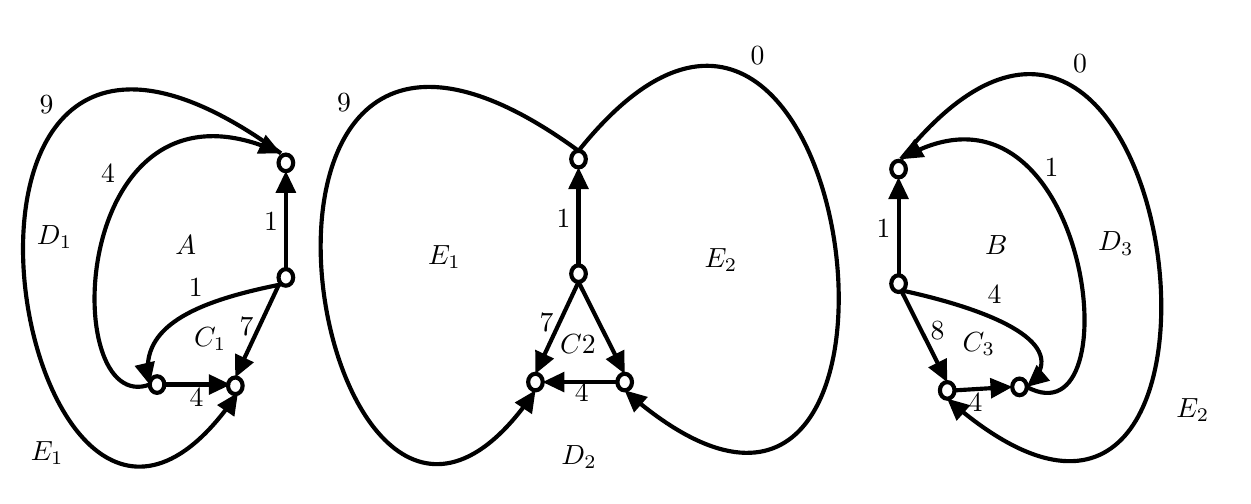
\begin{tikzpicture}[x=0.75pt,y=0.75pt,yscale=-0.9,xscale=0.9]
%uncomment if require: \path (0,498); %set diagram left start at 0, and has height of 498
\path[use as bounding box] (20,10) rectangle (660,250);
%Shape: Ellipse [id:dp012401419565516214] 
\draw  [color={rgb, 255:red, 0; green, 0; blue, 0 }  ,draw opacity=1 ][line width=1.5]  (310.98,80.38) .. controls (310.98,77.92) and (312.73,75.93) .. (314.89,75.93) .. controls (317.05,75.93) and (318.8,77.92) .. (318.8,80.38) .. controls (318.8,82.83) and (317.05,84.82) .. (314.89,84.82) .. controls (312.73,84.82) and (310.98,82.83) .. (310.98,80.38) -- cycle ;
%Shape: Ellipse [id:dp44563585877978507] 
\draw  [color={rgb, 255:red, 0; green, 0; blue, 0 }  ,draw opacity=1 ][line width=1.5]  (310.98,141.69) .. controls (310.98,139.23) and (312.73,137.24) .. (314.89,137.24) .. controls (317.05,137.24) and (318.8,139.23) .. (318.8,141.69) .. controls (318.8,144.14) and (317.05,146.13) .. (314.89,146.13) .. controls (312.73,146.13) and (310.98,144.14) .. (310.98,141.69) -- cycle ;
%Shape: Ellipse [id:dp8232398640866994] 
\draw  [color={rgb, 255:red, 0; green, 0; blue, 0 }  ,draw opacity=1 ][line width=1.5]  (287.92,199.72) .. controls (287.92,197.26) and (289.67,195.27) .. (291.83,195.27) .. controls (293.99,195.27) and (295.74,197.26) .. (295.74,199.72) .. controls (295.74,202.17) and (293.99,204.16) .. (291.83,204.16) .. controls (289.67,204.16) and (287.92,202.17) .. (287.92,199.72) -- cycle ;
%Shape: Ellipse [id:dp43325876938835506] 
\draw  [color={rgb, 255:red, 0; green, 0; blue, 0 }  ,draw opacity=1 ][line width=1.5]  (335.68,199.72) .. controls (335.68,197.26) and (337.44,195.27) .. (339.6,195.27) .. controls (341.76,195.27) and (343.51,197.26) .. (343.51,199.72) .. controls (343.51,202.17) and (341.76,204.16) .. (339.6,204.16) .. controls (337.44,204.16) and (335.68,202.17) .. (335.68,199.72) -- cycle ;
%Straight Lines [id:da24688497873734994] 
\draw [color={rgb, 255:red, 0; green, 0; blue, 0 }  ,draw opacity=1 ][line width=1.5]    (299.74,199.72) -- (335.68,199.72) ;
\draw [shift={(295.74,199.72)}, rotate = 0] [fill={rgb, 255:red, 0; green, 0; blue, 0 }  ,fill opacity=1 ][line width=0.08]  [draw opacity=0] (11.61,-5.58) -- (0,0) -- (11.61,5.58) -- cycle    ;
%Straight Lines [id:da9029001126541812] 
\draw [color={rgb, 255:red, 0; green, 0; blue, 0 }  ,draw opacity=1 ][line width=1.5]    (314.89,137.24) -- (314.89,88.82) ;
\draw [shift={(314.89,84.82)}, rotate = 90] [fill={rgb, 255:red, 0; green, 0; blue, 0 }  ,fill opacity=1 ][line width=0.08]  [draw opacity=0] (11.61,-5.58) -- (0,0) -- (11.61,5.58) -- cycle    ;
%Straight Lines [id:da22131359142153095] 
\draw [color={rgb, 255:red, 0; green, 0; blue, 0 }  ,draw opacity=1 ][line width=1.5]    (314.89,146.13) -- (293.53,191.65) ;
\draw [shift={(291.83,195.27)}, rotate = 295.14] [fill={rgb, 255:red, 0; green, 0; blue, 0 }  ,fill opacity=1 ][line width=0.08]  [draw opacity=0] (11.61,-5.58) -- (0,0) -- (11.61,5.58) -- cycle    ;
%Straight Lines [id:da6387841366636108] 
\draw [color={rgb, 255:red, 0; green, 0; blue, 0 }  ,draw opacity=1 ][line width=1.5]    (314.89,146.13) -- (337.8,191.7) ;
\draw [shift={(339.6,195.27)}, rotate = 243.31] [fill={rgb, 255:red, 0; green, 0; blue, 0 }  ,fill opacity=1 ][line width=0.08]  [draw opacity=0] (11.61,-5.58) -- (0,0) -- (11.61,5.58) -- cycle    ;
%Curve Lines [id:da15562696066606252] 
\draw [line width=1.5]    (314.89,75.93) .. controls (97.2,-83.01) and (174.77,372.56) .. (290.09,206.71) ;
\draw [shift={(291.83,204.16)}, rotate = 123.91] [fill={rgb, 255:red, 0; green, 0; blue, 0 }  ][line width=0.08]  [draw opacity=0] (11.61,-5.58) -- (0,0) -- (11.61,5.58) -- cycle    ;
%Curve Lines [id:da37566750523718095] 
\draw [line width=1.5]    (314.89,75.93) .. controls (466.51,-113.62) and (520.64,359.85) .. (342.3,206.52) ;
\draw [shift={(339.6,204.16)}, rotate = 41.47] [fill={rgb, 255:red, 0; green, 0; blue, 0 }  ][line width=0.08]  [draw opacity=0] (11.61,-5.58) -- (0,0) -- (11.61,5.58) -- cycle    ;
%Shape: Ellipse [id:dp2127358898052878] 
\draw  [color={rgb, 255:red, 0; green, 0; blue, 0 }  ,draw opacity=1 ][line width=1.5]  (85.35,201.05) .. controls (85.35,198.6) and (87.1,196.61) .. (89.26,196.61) .. controls (91.42,196.61) and (93.17,198.6) .. (93.17,201.05) .. controls (93.17,203.51) and (91.42,205.5) .. (89.26,205.5) .. controls (87.1,205.5) and (85.35,203.51) .. (85.35,201.05) -- cycle ;
%Curve Lines [id:da6892910775973166] 
\draw [color={rgb, 255:red, 0; green, 0; blue, 0 }  ,draw opacity=1 ][line width=1.5]    (84.57,196.85) .. controls (81.15,170.86) and (107.05,157.02) .. (155.56,147.47) ;
\draw [shift={(85.35,201.05)}, rotate = 256.57] [fill={rgb, 255:red, 0; green, 0; blue, 0 }  ,fill opacity=1 ][line width=0.08]  [draw opacity=0] (11.61,-5.58) -- (0,0) -- (11.61,5.58) -- cycle    ;
%Curve Lines [id:da5288751216338294] 
\draw [color={rgb, 255:red, 0; green, 0; blue, 0 }  ,draw opacity=1 ][line width=1.5]    (85.35,201.05) .. controls (36.23,219.12) and (41.79,28.03) .. (152.18,75.75) ;
\draw [shift={(155.56,77.27)}, rotate = 205.05] [fill={rgb, 255:red, 0; green, 0; blue, 0 }  ,fill opacity=1 ][line width=0.08]  [draw opacity=0] (11.61,-5.58) -- (0,0) -- (11.61,5.58) -- cycle    ;
%Straight Lines [id:da24276479087471536] 
\draw [color={rgb, 255:red, 0; green, 0; blue, 0 }  ,draw opacity=1 ][line width=1.5]    (93.17,201.05) -- (124.59,201.05) ;
\draw [shift={(128.59,201.05)}, rotate = 180] [fill={rgb, 255:red, 0; green, 0; blue, 0 }  ,fill opacity=1 ][line width=0.08]  [draw opacity=0] (11.61,-5.58) -- (0,0) -- (11.61,5.58) -- cycle    ;
%Curve Lines [id:da32788257215994565] 
\draw [line width=1.5]    (155.56,77.27) .. controls (-62.14,-81.67) and (15.44,373.9) .. (130.76,208.05) ;
\draw [shift={(132.5,205.5)}, rotate = 123.91] [fill={rgb, 255:red, 0; green, 0; blue, 0 }  ][line width=0.08]  [draw opacity=0] (11.61,-5.58) -- (0,0) -- (11.61,5.58) -- cycle    ;
%Shape: Ellipse [id:dp4018621662081351] 
\draw  [color={rgb, 255:red, 0; green, 0; blue, 0 }  ,draw opacity=1 ][line width=1.5]  (127.25,201.72) .. controls (127.25,199.26) and (129,197.27) .. (131.16,197.27) .. controls (133.32,197.27) and (135.08,199.26) .. (135.08,201.72) .. controls (135.08,204.17) and (133.32,206.16) .. (131.16,206.16) .. controls (129,206.16) and (127.25,204.17) .. (127.25,201.72) -- cycle ;
%Straight Lines [id:da06341837878705825] 
\draw [color={rgb, 255:red, 0; green, 0; blue, 0 }  ,draw opacity=1 ][line width=1.5]    (154.22,148.13) -- (132.86,193.65) ;
\draw [shift={(131.16,197.27)}, rotate = 295.14] [fill={rgb, 255:red, 0; green, 0; blue, 0 }  ,fill opacity=1 ][line width=0.08]  [draw opacity=0] (11.61,-5.58) -- (0,0) -- (11.61,5.58) -- cycle    ;
%Shape: Ellipse [id:dp38906306008016145] 
\draw  [color={rgb, 255:red, 0; green, 0; blue, 0 }  ,draw opacity=1 ][line width=1.5]  (154.31,82.38) .. controls (154.31,79.92) and (156.06,77.93) .. (158.22,77.93) .. controls (160.38,77.93) and (162.14,79.92) .. (162.14,82.38) .. controls (162.14,84.83) and (160.38,86.82) .. (158.22,86.82) .. controls (156.06,86.82) and (154.31,84.83) .. (154.31,82.38) -- cycle ;
%Shape: Ellipse [id:dp08743735948745213] 
\draw  [color={rgb, 255:red, 0; green, 0; blue, 0 }  ,draw opacity=1 ][line width=1.5]  (154.31,143.69) .. controls (154.31,141.23) and (156.06,139.24) .. (158.22,139.24) .. controls (160.38,139.24) and (162.14,141.23) .. (162.14,143.69) .. controls (162.14,146.14) and (160.38,148.13) .. (158.22,148.13) .. controls (156.06,148.13) and (154.31,146.14) .. (154.31,143.69) -- cycle ;
%Straight Lines [id:da6699514353142748] 
\draw [color={rgb, 255:red, 0; green, 0; blue, 0 }  ,draw opacity=1 ][line width=1.5]    (158.22,139.24) -- (158.22,90.82) ;
\draw [shift={(158.22,86.82)}, rotate = 90] [fill={rgb, 255:red, 0; green, 0; blue, 0 }  ,fill opacity=1 ][line width=0.08]  [draw opacity=0] (11.61,-5.58) -- (0,0) -- (11.61,5.58) -- cycle    ;
%Shape: Ellipse [id:dp8050348596658142] 
\draw  [color={rgb, 255:red, 0; green, 0; blue, 0 }  ,draw opacity=1 ][line width=1.5]  (547.06,202.3) .. controls (547.06,199.84) and (548.81,197.85) .. (550.97,197.85) .. controls (553.13,197.85) and (554.88,199.84) .. (554.88,202.3) .. controls (554.88,204.75) and (553.13,206.75) .. (550.97,206.75) .. controls (548.81,206.75) and (547.06,204.75) .. (547.06,202.3) -- cycle ;
%Shape: Ellipse [id:dp4814843770420125] 
\draw  [color={rgb, 255:red, 0; green, 0; blue, 0 }  ,draw opacity=1 ][line width=1.5]  (508.35,204.17) .. controls (508.35,201.72) and (510.1,199.73) .. (512.26,199.73) .. controls (514.42,199.73) and (516.18,201.72) .. (516.18,204.17) .. controls (516.18,206.63) and (514.42,208.62) .. (512.26,208.62) .. controls (510.1,208.62) and (508.35,206.63) .. (508.35,204.17) -- cycle ;
%Curve Lines [id:da6756687162833178] 
\draw [color={rgb, 255:red, 0; green, 0; blue, 0 }  ,draw opacity=1 ][line width=1.5]    (557.85,199.47) .. controls (576.23,179.57) and (540.25,161.98) .. (487.56,150.59) ;
\draw [shift={(554.88,202.3)}, rotate = 319.56] [fill={rgb, 255:red, 0; green, 0; blue, 0 }  ,fill opacity=1 ][line width=0.08]  [draw opacity=0] (11.61,-5.58) -- (0,0) -- (11.61,5.58) -- cycle    ;
%Curve Lines [id:da3167596918642579] 
\draw [color={rgb, 255:red, 0; green, 0; blue, 0 }  ,draw opacity=1 ][line width=1.5]    (554.88,202.3) .. controls (612.57,233.81) and (588.52,24.96) .. (490.55,78.68) ;
\draw [shift={(487.56,80.38)}, rotate = 329.29] [fill={rgb, 255:red, 0; green, 0; blue, 0 }  ,fill opacity=1 ][line width=0.08]  [draw opacity=0] (11.61,-5.58) -- (0,0) -- (11.61,5.58) -- cycle    ;
%Straight Lines [id:da5914875377963786] 
\draw [color={rgb, 255:red, 0; green, 0; blue, 0 }  ,draw opacity=1 ][line width=1.5]    (516.18,204.17) -- (543.07,202.54) ;
\draw [shift={(547.06,202.3)}, rotate = 176.53] [fill={rgb, 255:red, 0; green, 0; blue, 0 }  ,fill opacity=1 ][line width=0.08]  [draw opacity=0] (11.61,-5.58) -- (0,0) -- (11.61,5.58) -- cycle    ;
%Straight Lines [id:da07161147378506905] 
\draw [color={rgb, 255:red, 0; green, 0; blue, 0 }  ,draw opacity=1 ][line width=1.5]    (487.56,150.59) -- (510.47,196.15) ;
\draw [shift={(512.26,199.73)}, rotate = 243.31] [fill={rgb, 255:red, 0; green, 0; blue, 0 }  ,fill opacity=1 ][line width=0.08]  [draw opacity=0] (11.61,-5.58) -- (0,0) -- (11.61,5.58) -- cycle    ;
%Curve Lines [id:da5080118287083738] 
\draw [line width=1.5]    (487.56,80.38) .. controls (639.17,-109.17) and (693.31,364.3) .. (514.97,210.98) ;
\draw [shift={(512.26,208.62)}, rotate = 41.47] [fill={rgb, 255:red, 0; green, 0; blue, 0 }  ][line width=0.08]  [draw opacity=0] (11.61,-5.58) -- (0,0) -- (11.61,5.58) -- cycle    ;
%Shape: Ellipse [id:dp8095971328672295] 
\draw  [color={rgb, 255:red, 0; green, 0; blue, 0 }  ,draw opacity=1 ][line width=1.5]  (482.31,85.71) .. controls (482.31,83.26) and (484.06,81.27) .. (486.22,81.27) .. controls (488.38,81.27) and (490.14,83.26) .. (490.14,85.71) .. controls (490.14,88.17) and (488.38,90.16) .. (486.22,90.16) .. controls (484.06,90.16) and (482.31,88.17) .. (482.31,85.71) -- cycle ;
%Shape: Ellipse [id:dp915558520007347] 
\draw  [color={rgb, 255:red, 0; green, 0; blue, 0 }  ,draw opacity=1 ][line width=1.5]  (482.31,147.02) .. controls (482.31,144.56) and (484.06,142.57) .. (486.22,142.57) .. controls (488.38,142.57) and (490.14,144.56) .. (490.14,147.02) .. controls (490.14,149.47) and (488.38,151.47) .. (486.22,151.47) .. controls (484.06,151.47) and (482.31,149.47) .. (482.31,147.02) -- cycle ;
%Straight Lines [id:da8569739762561568] 
\draw [color={rgb, 255:red, 0; green, 0; blue, 0 }  ,draw opacity=1 ][line width=1.5]    (486.22,142.57) -- (486.22,94.16) ;
\draw [shift={(486.22,90.16)}, rotate = 90] [fill={rgb, 255:red, 0; green, 0; blue, 0 }  ,fill opacity=1 ][line width=0.08]  [draw opacity=0] (11.61,-5.58) -- (0,0) -- (11.61,5.58) -- cycle    ;

% Text Node
\draw (311.27,198.94) node [anchor=north west][inner sep=0.75pt]    {$4$};
% Text Node
\draw (301.54,105.56) node [anchor=north west][inner sep=0.75pt]    {$1$};
% Text Node
\draw (303.43,172.5) node [anchor=north west][inner sep=0.75pt]    {$C2$};
% Text Node
\draw (304.1,231.81) node [anchor=north west][inner sep=0.75pt]    {$D_{2}$};
% Text Node
\draw (184.03,43.64) node [anchor=north west][inner sep=0.75pt]    {$9$};
% Text Node
\draw (405.37,18.28) node [anchor=north west][inner sep=0.75pt]    {$0$};
% Text Node
\draw (292.43,161.58) node [anchor=north west][inner sep=0.75pt]    {$7$};
% Text Node
\draw (97.44,119.41) node [anchor=north west][inner sep=0.75pt]    {$A$};
% Text Node
\draw (23.28,114.24) node [anchor=north west][inner sep=0.75pt]    {$D_{1}$};
% Text Node
\draw (104.58,142.94) node [anchor=north west][inner sep=0.75pt]    {$1$};
% Text Node
\draw (57.66,81.61) node [anchor=north west][inner sep=0.75pt]    {$4$};
% Text Node
\draw (105.02,201.78) node [anchor=north west][inner sep=0.75pt]    {$4$};
% Text Node
\draw (107.45,168.75) node [anchor=north west][inner sep=0.75pt]    {$C_{1}$};
% Text Node
\draw (24.7,44.97) node [anchor=north west][inner sep=0.75pt]    {$9$};
% Text Node
\draw (131.76,163.58) node [anchor=north west][inner sep=0.75pt]    {$7$};
% Text Node
\draw (144.87,107.56) node [anchor=north west][inner sep=0.75pt]    {$1$};
% Text Node
\draw (633.33,207.07) node [anchor=north west][inner sep=0.75pt]    {$E_{2}$};
% Text Node
\draw (380.67,126.4) node [anchor=north west][inner sep=0.75pt]    {$E_{2}$};
% Text Node
\draw (530.86,119.53) node [anchor=north west][inner sep=0.75pt]    {$B$};
% Text Node
\draw (562.73,78.22) node [anchor=north west][inner sep=0.75pt]    {$1$};
% Text Node
\draw (532.19,146.31) node [anchor=north west][inner sep=0.75pt]    {$4$};
% Text Node
\draw (522.01,204.4) node [anchor=north west][inner sep=0.75pt]    {$4$};
% Text Node
\draw (518.91,171.59) node [anchor=north west][inner sep=0.75pt]    {$C_{3}$};
% Text Node
\draw (591.4,117.74) node [anchor=north west][inner sep=0.75pt]    {$D_{3}$};
% Text Node
\draw (578.03,22.73) node [anchor=north west][inner sep=0.75pt]    {$0$};
% Text Node
\draw (501.7,165.47) node [anchor=north west][inner sep=0.75pt]    {$8$};
% Text Node
\draw (472.87,110.89) node [anchor=north west][inner sep=0.75pt]    {$1$};
% Text Node
\draw (232.67,125.07) node [anchor=north west][inner sep=0.75pt]    {$E_{1}$};
% Text Node
\draw (20,229.73) node [anchor=north west][inner sep=0.75pt]    {$E_{1}$};


\end{tikzpicture}